\chapter{Part II(b) - Processor, I/Os, and Exceptions W - 4.2}
\section{The CPU}

The CPU is a very sequential component responsible for executing instructions in a controlled manner. The CPU interacts with the memory through a defined memory interface, which includes various control signals and data pathways.
\begin{center}
    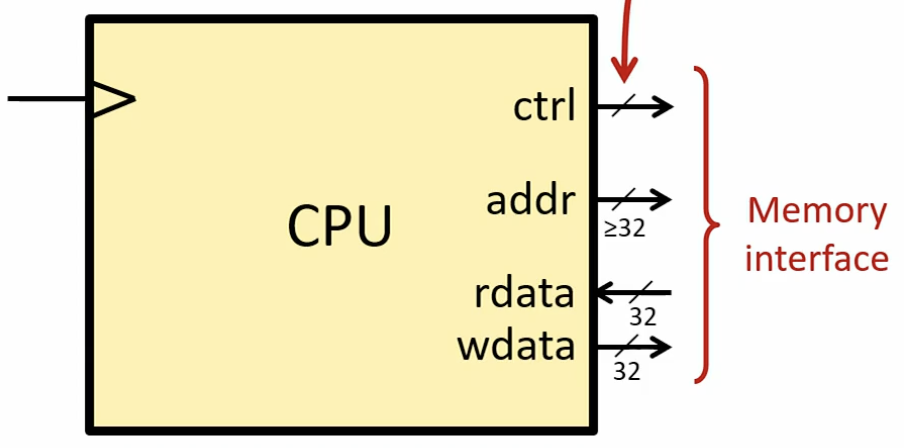
\includegraphics[width=0.45\textwidth]{chapters/chapter2b/images/cpu.png}
\end{center}
\begin{itemize}
    \item[-] \textbf{Control Signals (ctrl)}: These signals manage the behavior of memory access, indicating whether to read or write data.
    \item[-] \textbf{Address (addr)}: Specifies the memory address where the CPU wants to read or write data. The width of the address bus is typically 32 bits or more.
    \item[-] \textbf{Read Data (rdata)}: A 32-bit pathway through which the CPU receives data from the memory.
    \item[-] \textbf{Write Data (wdata)}: A 32-bit pathway through which the CPU sends data to be stored in memory.
\end{itemize}

The memory interface is also controlled by two important signals:
\begin{itemize}
    \item[-] \textbf{Circuit Enable (CE)}: Validates the address, indicating that the address provided is active and the operation should proceed.
    \item[-] \textbf{Write Enable (WE)}: Indicates that the current access is a store operation, allowing data to be written into memory.
\end{itemize}
\textbf{From now on, the clock signal, which drives the sequential behavior, may be omitted for simplicity.}
This interface design allows for a clear and structured method of communication between the CPU and memory, ensuring reliable execution of instructions and data management.



